% nitu_spin.tex -- insert with % nitu_spin.tex -- insert with % nitu_spin.tex -- insert with % nitu_spin.tex -- insert with \input{nitu_spin} at the end of the Method D section (just before \section{Testing the Methods}).
\subsection{What the observations reveal about the spin}
Figure~\ref{fig:spinpost} compares the prior and the likelihood-weighted posterior of the ensemble. The two observations shift the spin rate towards higher values (curve-kick range) and favour a spin axis that bends the ball towards the centre of the goal. The right panel shows why the lateral entry point is uncertain: $y_{\rm goal}$ is almost a linear function of the vertical component of the spin axis, i.e.\ of the amount of sidespin, which the first 0.10 s constrain only weakly. The weighted distribution of $y_{\rm goal}$ is therefore bimodal (curve and instep draws), while that of $z_{\rm goal}$ has a single peak (Figure~\ref{fig:marg}).

\begin{figure}[H]
  \centering
  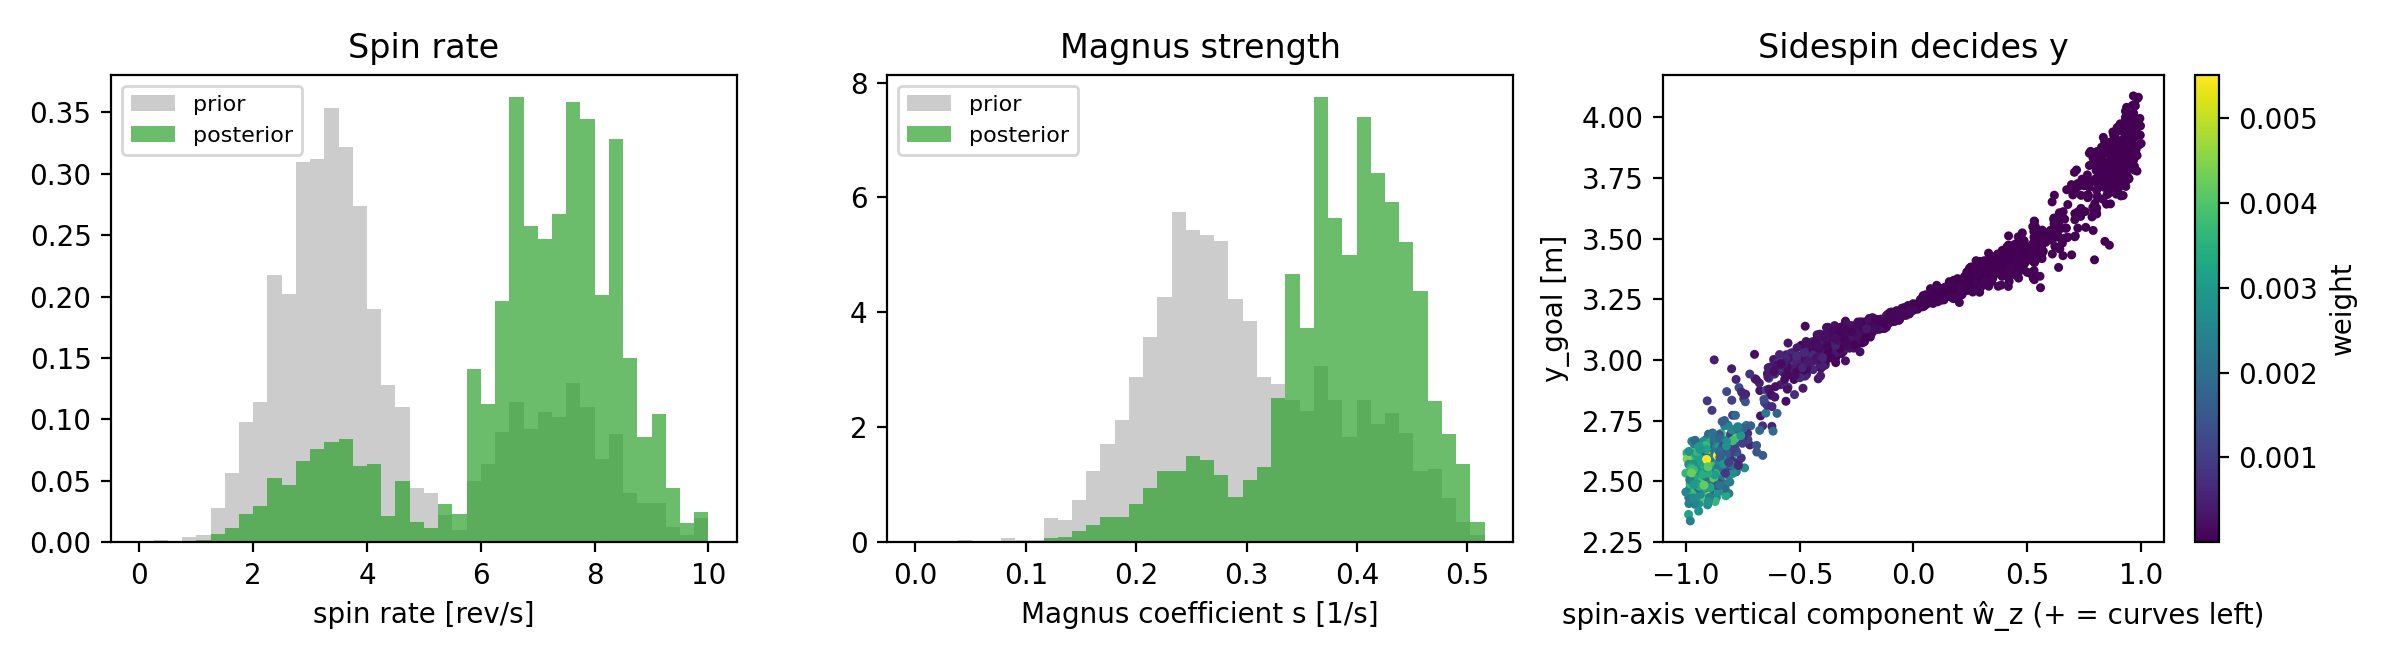
\includegraphics[width=\linewidth]{../penalty_dataset_v3/Model-D/fig_spin_posterior.png}
  \caption{Prior (grey) and posterior (green) of the spin rate and Magnus strength, and the dependence of the lateral entry point on the sidespin component of the spin axis (colour: weight).}
  \label{fig:spinpost}
\end{figure}

\begin{figure}[H]
  \centering
  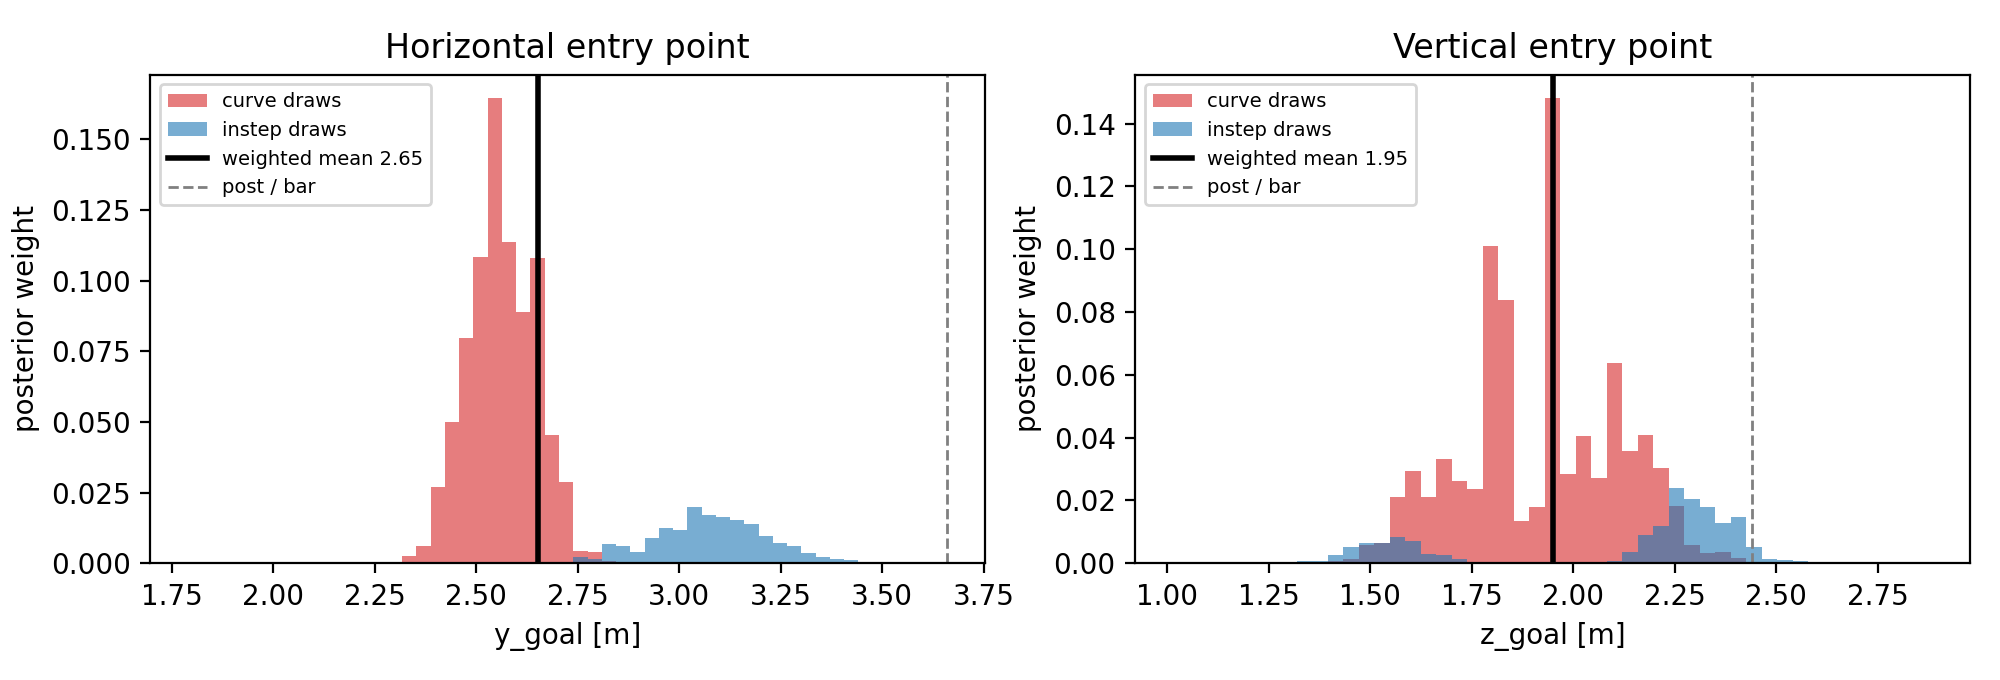
\includegraphics[width=\linewidth]{../penalty_dataset_v3/Model-D/fig_marginals.png}
  \caption{Weighted distributions of the entry point for the given shot, split into curve-kick and instep draws.}
  \label{fig:marg}
\end{figure}
 at the end of the Method D section (just before \section{Testing the Methods}).
\subsection{What the observations reveal about the spin}
Figure~\ref{fig:spinpost} compares the prior and the likelihood-weighted posterior of the ensemble. The two observations shift the spin rate towards higher values (curve-kick range) and favour a spin axis that bends the ball towards the centre of the goal. The right panel shows why the lateral entry point is uncertain: $y_{\rm goal}$ is almost a linear function of the vertical component of the spin axis, i.e.\ of the amount of sidespin, which the first 0.10 s constrain only weakly. The weighted distribution of $y_{\rm goal}$ is therefore bimodal (curve and instep draws), while that of $z_{\rm goal}$ has a single peak (Figure~\ref{fig:marg}).

\begin{figure}[H]
  \centering
  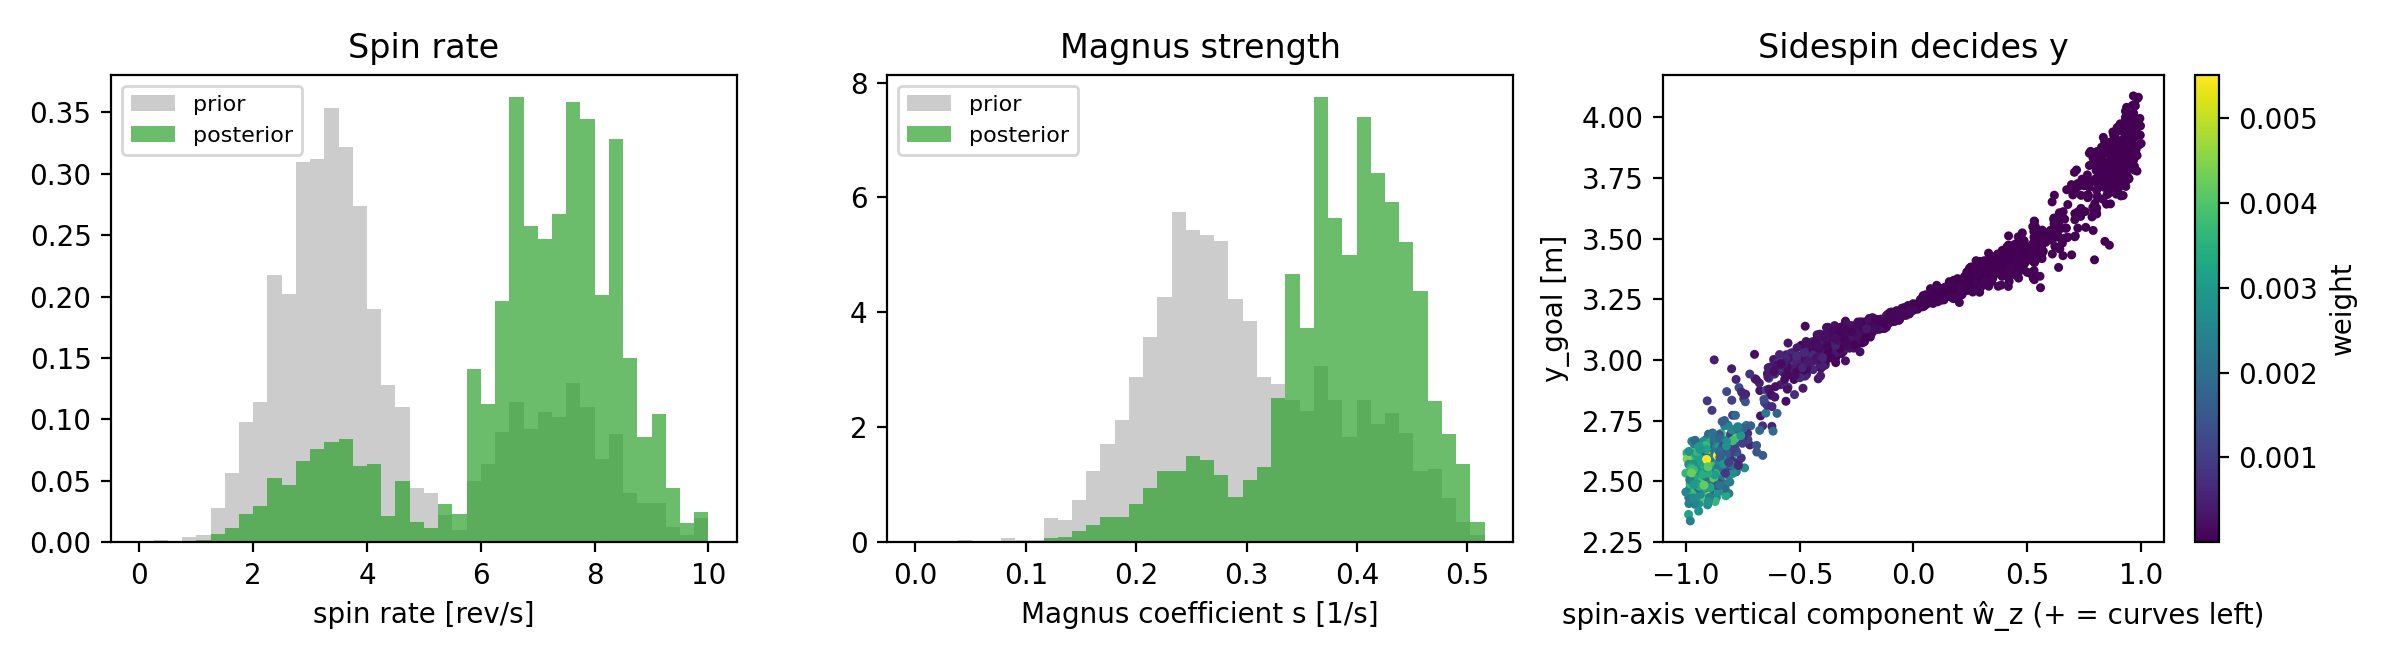
\includegraphics[width=\linewidth]{../penalty_dataset_v3/Model-D/fig_spin_posterior.png}
  \caption{Prior (grey) and posterior (green) of the spin rate and Magnus strength, and the dependence of the lateral entry point on the sidespin component of the spin axis (colour: weight).}
  \label{fig:spinpost}
\end{figure}

\begin{figure}[H]
  \centering
  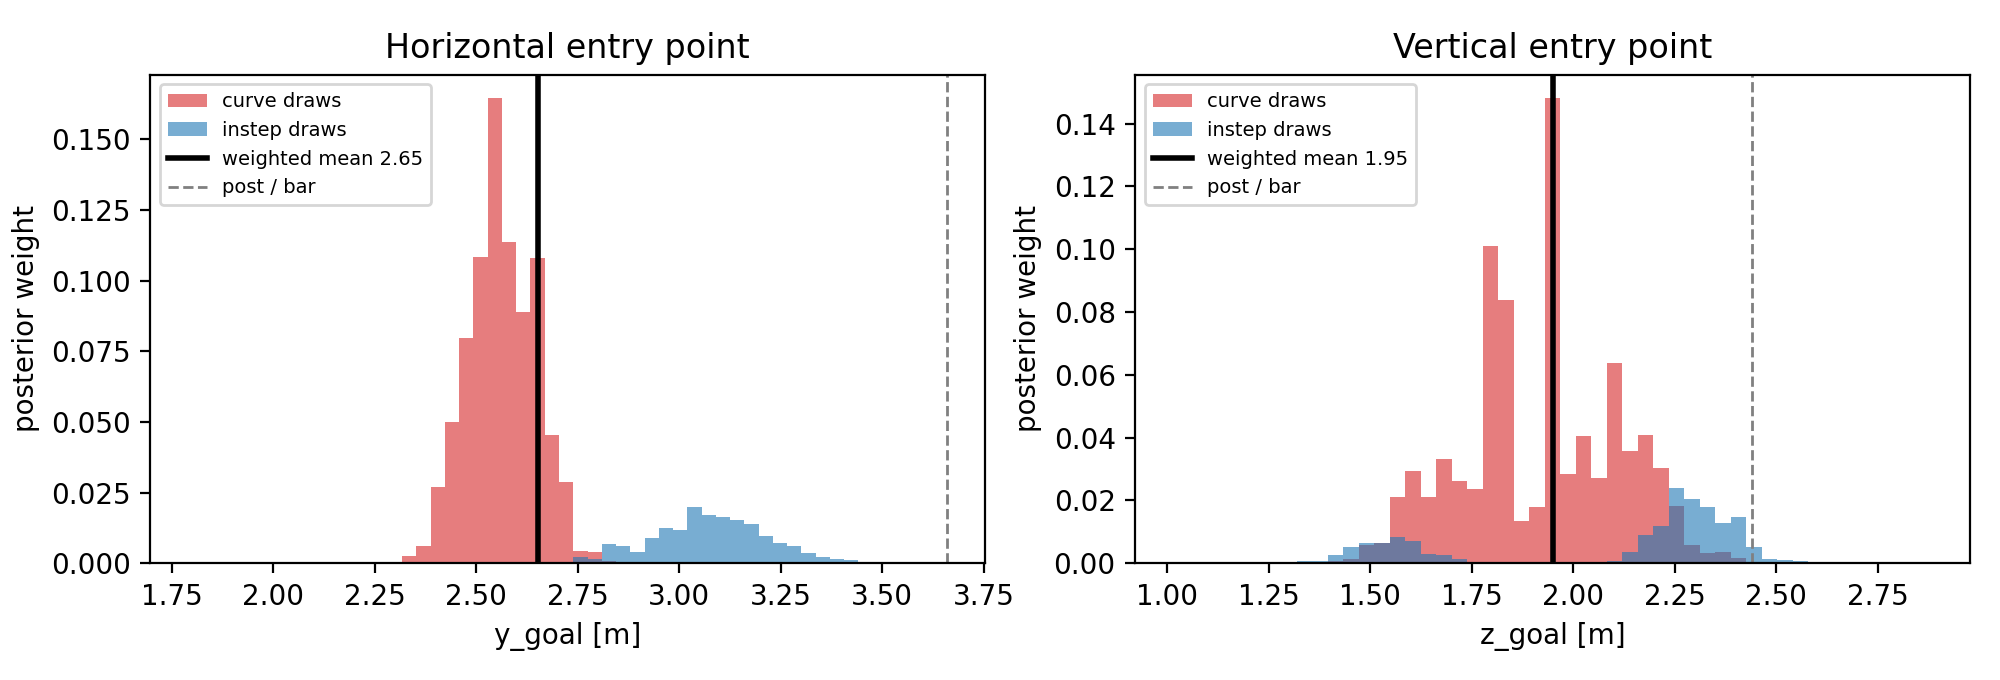
\includegraphics[width=\linewidth]{../penalty_dataset_v3/Model-D/fig_marginals.png}
  \caption{Weighted distributions of the entry point for the given shot, split into curve-kick and instep draws.}
  \label{fig:marg}
\end{figure}
 at the end of the Method D section (just before \section{Testing the Methods}).
\subsection{What the observations reveal about the spin}
Figure~\ref{fig:spinpost} compares the prior and the likelihood-weighted posterior of the ensemble. The two observations shift the spin rate towards higher values (curve-kick range) and favour a spin axis that bends the ball towards the centre of the goal. The right panel shows why the lateral entry point is uncertain: $y_{\rm goal}$ is almost a linear function of the vertical component of the spin axis, i.e.\ of the amount of sidespin, which the first 0.10 s constrain only weakly. The weighted distribution of $y_{\rm goal}$ is therefore bimodal (curve and instep draws), while that of $z_{\rm goal}$ has a single peak (Figure~\ref{fig:marg}).

\begin{figure}[H]
  \centering
  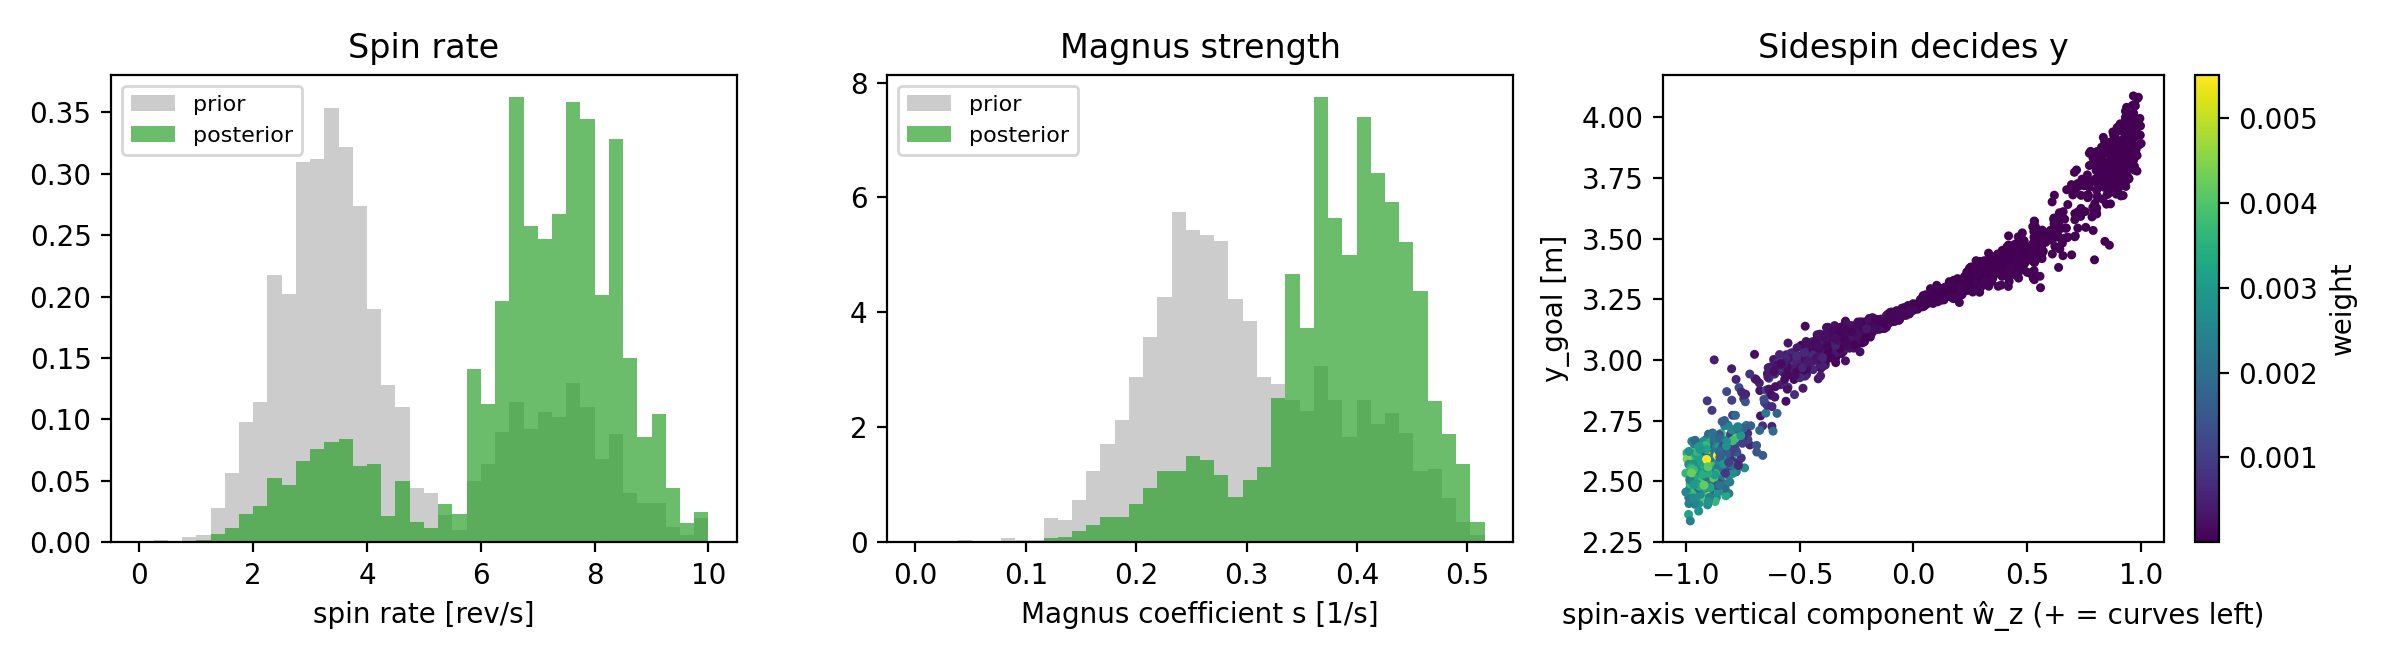
\includegraphics[width=\linewidth]{../penalty_dataset_v3/Model-D/fig_spin_posterior.png}
  \caption{Prior (grey) and posterior (green) of the spin rate and Magnus strength, and the dependence of the lateral entry point on the sidespin component of the spin axis (colour: weight).}
  \label{fig:spinpost}
\end{figure}

\begin{figure}[H]
  \centering
  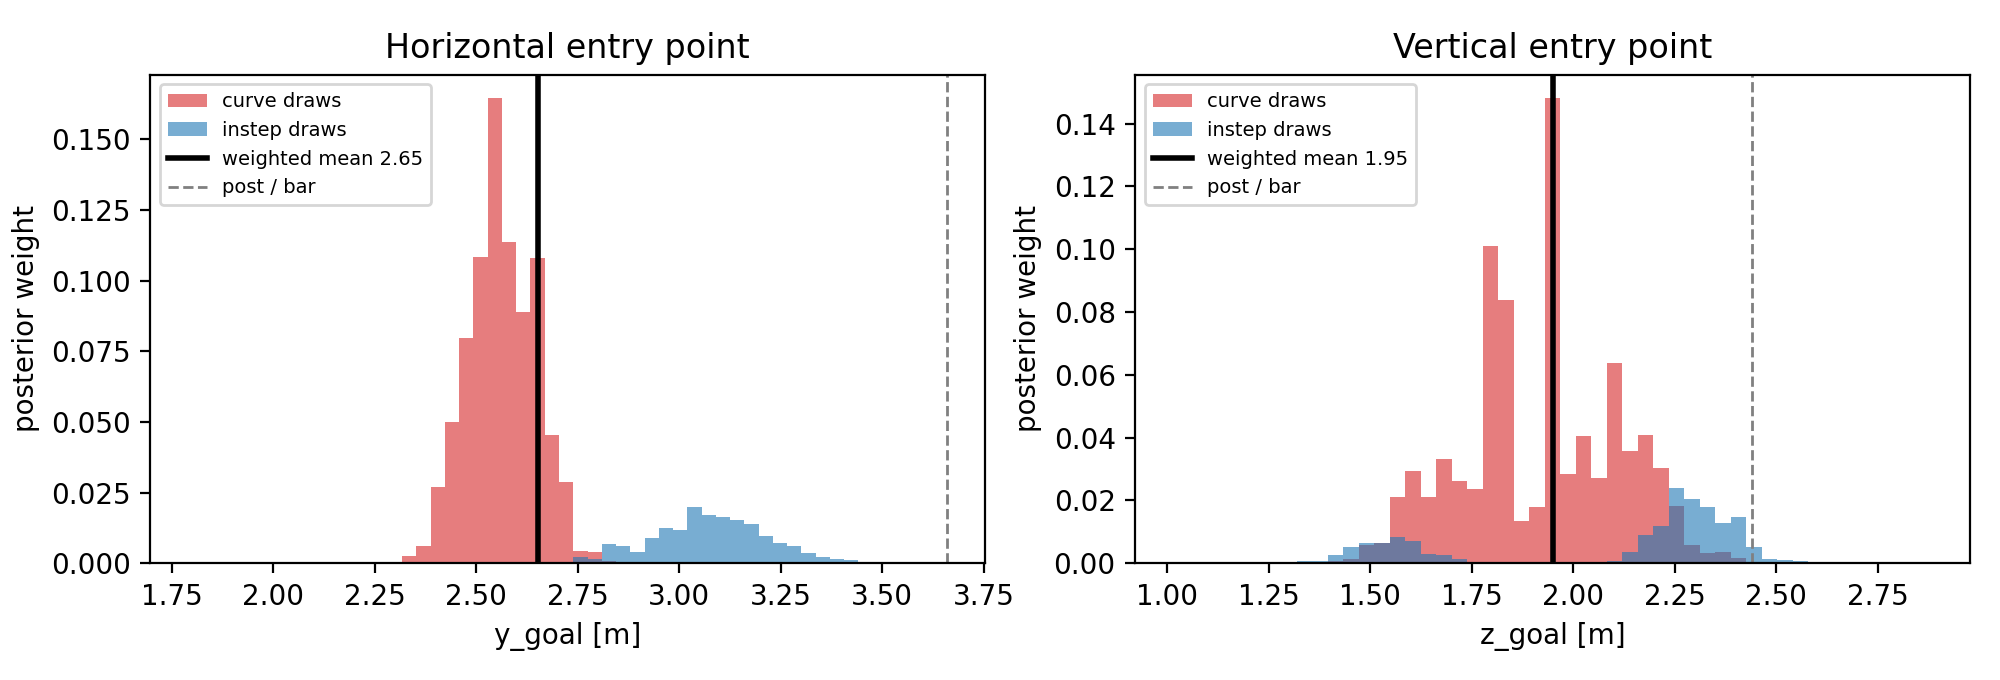
\includegraphics[width=\linewidth]{../penalty_dataset_v3/Model-D/fig_marginals.png}
  \caption{Weighted distributions of the entry point for the given shot, split into curve-kick and instep draws.}
  \label{fig:marg}
\end{figure}
 at the end of the Method D section (just before \section{Testing the Methods}).
\subsection{What the observations reveal about the spin}
Figure~\ref{fig:spinpost} compares the prior and the likelihood-weighted posterior of the ensemble. The two observations shift the spin rate towards higher values (curve-kick range) and favour a spin axis that bends the ball towards the centre of the goal. The right panel shows why the lateral entry point is uncertain: $y_{\rm goal}$ is almost a linear function of the vertical component of the spin axis, i.e.\ of the amount of sidespin, which the first 0.10 s constrain only weakly. The weighted distribution of $y_{\rm goal}$ is therefore bimodal (curve and instep draws), while that of $z_{\rm goal}$ has a single peak (Figure~\ref{fig:marg}).

\begin{figure}[H]
  \centering
  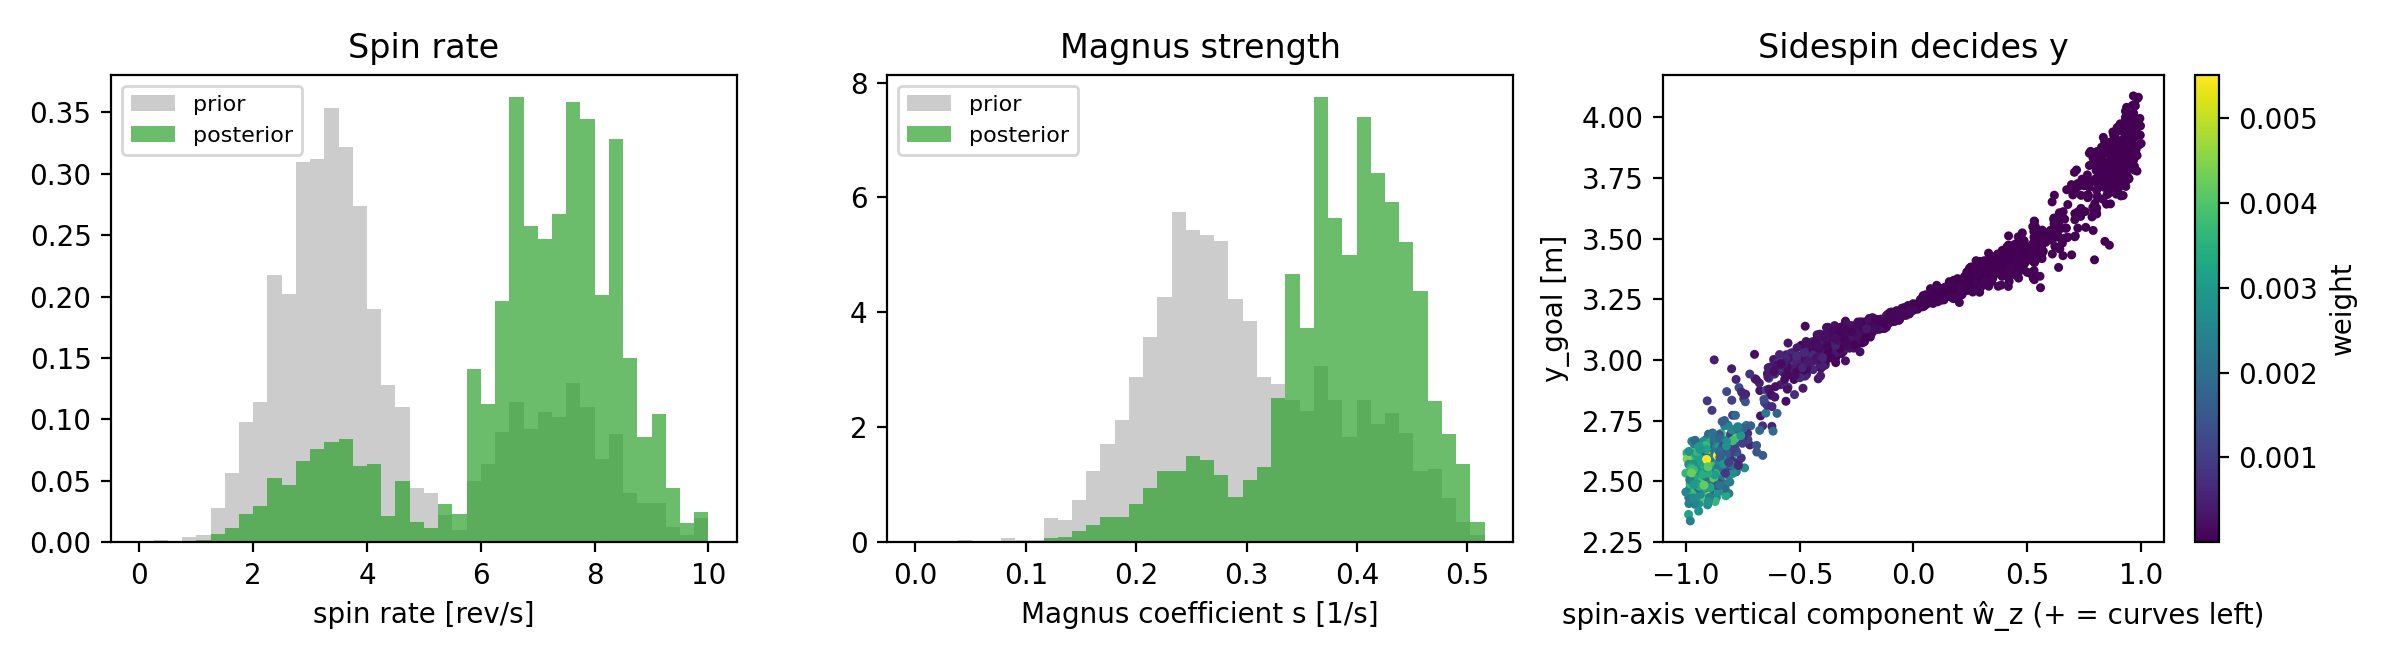
\includegraphics[width=\linewidth]{../penalty_dataset_v3/Model-D/fig_spin_posterior.png}
  \caption{Prior (grey) and posterior (green) of the spin rate and Magnus strength, and the dependence of the lateral entry point on the sidespin component of the spin axis (colour: weight).}
  \label{fig:spinpost}
\end{figure}

\begin{figure}[H]
  \centering
  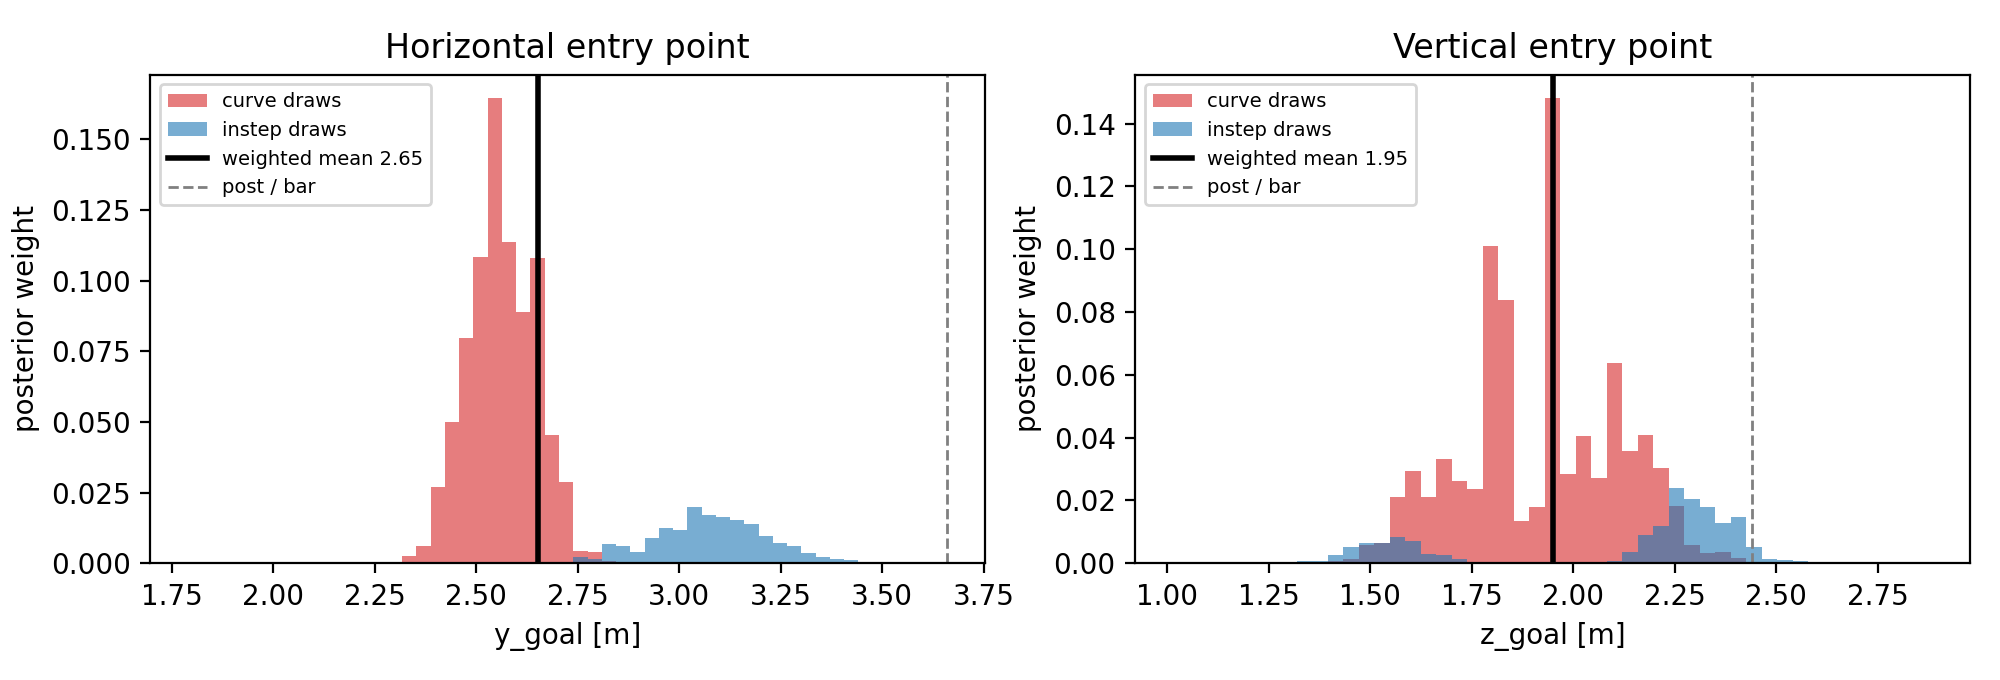
\includegraphics[width=\linewidth]{../penalty_dataset_v3/Model-D/fig_marginals.png}
  \caption{Weighted distributions of the entry point for the given shot, split into curve-kick and instep draws.}
  \label{fig:marg}
\end{figure}
